\chapter{Конструкторский раздел}

В этом разделе будет представлено описание используемых типов данных, а также схематические изображения алгоритмов сортировок: блочной, быстрой и выбором.

\section{Требования к программному обеспечению}

Программа должна поддерживать два режима работы: режим массового замера времени и режим сортировки введенного массива.

Режим массового замера времени должен обладать следующей функциональностью:
\begin{itemize}
	\item генерировать массивы различного размер для проведения замеров;
	\item осуществлять массовый замер, используя сгенерированные данные;
	\item результаты массового замера должны быть представлены в виде таблицы и графика.
\end{itemize}

К режиму сортировки выдвигается следующий ряд требований:
\begin{itemize}
	\item возможность работать с массивами разного размера, которые вводит пользователь;
	\item наличие интерфейса для выбора действий;
	\item на выходе программы массив, отсортированный тремя алгоритмами по возрастанию.
\end{itemize}

\section{Описание используемых типов данных}

При реализации алгоритмов будут использованы следующие структуры и типы данных:
\begin{itemize}
	\item целое число представляет количество элементов в массиве;
	\item массив целых чисел;
\end{itemize}

\section{Разработка алгоритмов}

На рисунке \ref{pic:blocksort} приведена схема алгоритма блочной сортировки.

\begin{figure}[H]
	\centering
	
\includegraphics[scale=0.62]{assets/blocksort.pdf}
	\caption{Схема алгоритма блочной сортировки}
	\label{pic:blocksort}
\end{figure}

\newpage

На рисунке \ref{pic:quicksort} приведена схема алгоритма быстрой сортировки.

\begin{figure}[H]
	\centering
	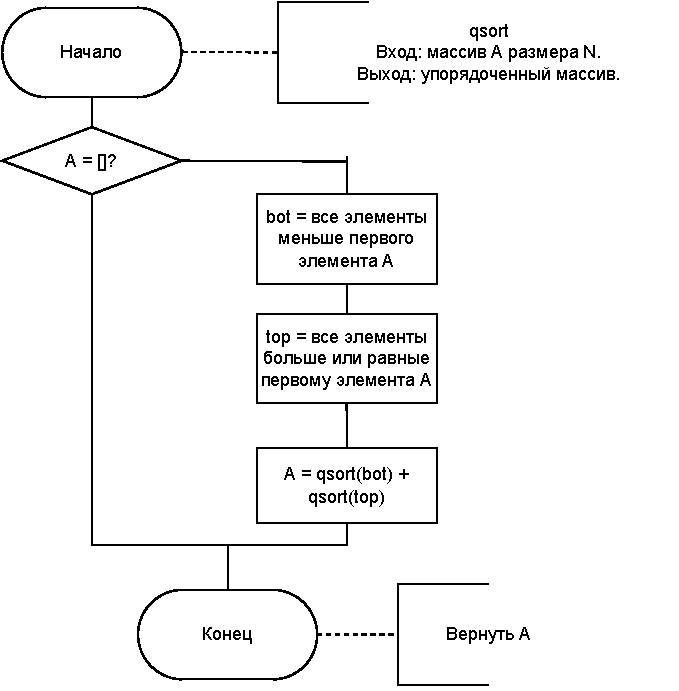
\includegraphics[scale=0.62]{assets/quicksort.pdf}
	\caption{Схема алгоритма быстрой сортировки}
	\label{pic:quicksort}
\end{figure}

\newpage

На рисунке \ref{pic:selectionsort} приведена схема алгоритма сортировки выбором.

\begin{figure}[H]
	\centering
	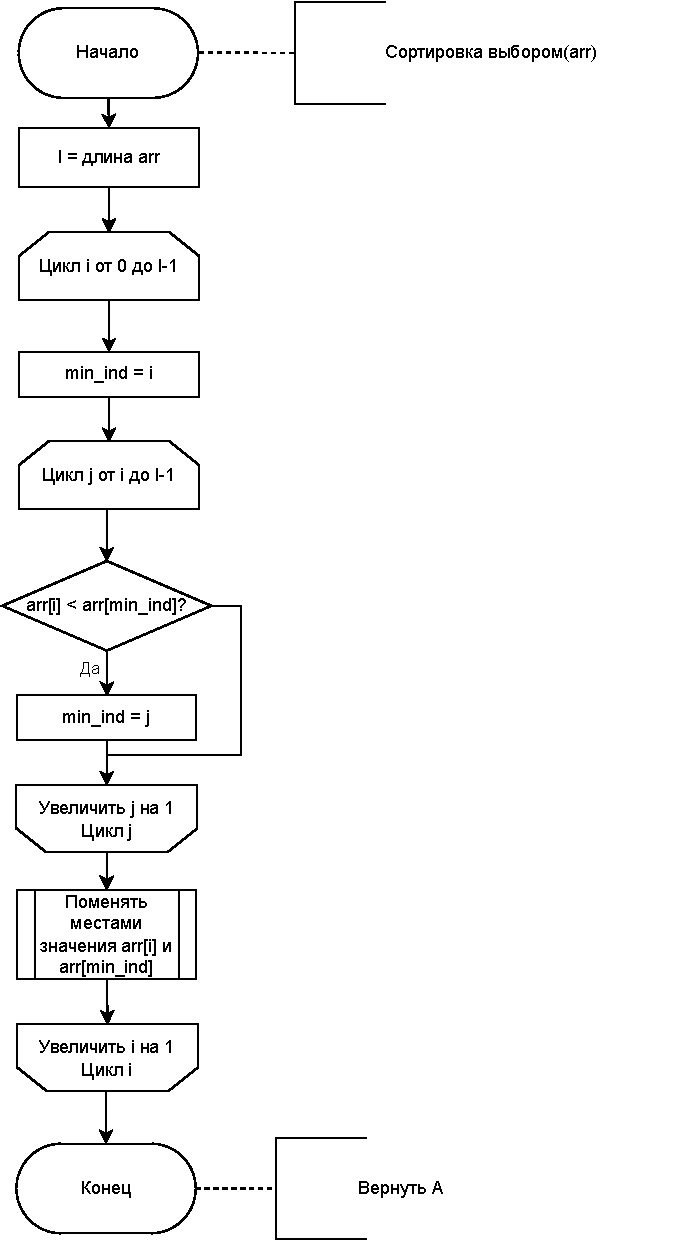
\includegraphics[scale=0.62]{assets/selectionsort.pdf}
	\caption{Схема алгоритма сортировки выбором}
	\label{pic:selectionsort}
\end{figure}

\newpage


\section{Оценка трудоемкости алгоритмов}

Модель для оценки трудоемкости алгоритмов состоит из шести пунктов:
\begin{enumerate}
	\item $+, -, =, +=, -=, ==, ||, \&\&, <, >, <=, >=, <<, >>, []$ --- считается, что эти операции обладают трудоемкостью в 1 единицу;
	\item $*, /, *=, /=, \% $ --- считается, что эти операции обладают трудоемкостью в 2 единицы;
	\item трудоемкость условного перехода принимается за $0$;
	\item трудоемкость условного оператора рассчитывается по формуле \eqref{eq:if},
	\begin{equation}
		\label{eq:if}
		f_{if} = f_{\text{условия}} + 
		\begin{cases}
			min(f_1, f_2), & \text{лучший случай}\\
			max(f_1, f_2), & \text{худший случай}
		\end{cases},
	\end{equation}
	где $f_1$ --- трудоемкость блока, который вычисляется при выполнении условия, а $f_2$ --- трудоемкость блока, который вычисляется при невыполнении условия;
	\item трудоемкость цикла рассчитывается по формуле \eqref{eq:for},
	\begin{equation}
		\label{eq:for}
		\begin{gathered}
			f_{for} = f_{\text{инициализация}} + f_{\text{сравнения}} + M_{\text{итераций}} \cdot (f_{\text{тело}} +\\
			+ f_{\text{инкремент}} + f_{\text{сравнения}});
		\end{gathered}
	\end{equation}
	\item вызов подпрограмм и передача параметров принимается за $0$.
\end{enumerate}

\subsection{Трудоемкость алгоритма Шелла}

При расчете трудоемкости считается, что $\lfloor \log_{2}N \rfloor \approx \log_{2}N $.
В лучшем случае, когда массив отсортирован трудоемкость алгоритма Шелла рассчитывается по формуле \eqref{eq:shell_best}.
\begin{equation}
	\label{eq:shell_best}
	\begin{gathered}
		f_{best} = 10 N \log_{2}N - 10 N + 5 \log_{2}N + 14 \approx O(N\log_{2}N)
	\end{gathered}
\end{equation}
 
В худшем случае, когда переставляются элементы во всех итерациях, трудоемкость алгоритма Шелла рассчитывается по формуле \eqref{eq:shell_worst}.
\begin{equation}
	\label{eq:shell_worst}
	\begin{gathered}
		f_{worst} = \frac{32}{3}N^2 + 10 N \log_{2}N - 26 N + 5 \log_{2}N + \frac{58}{3} \approx O(N^2)
	\end{gathered}
\end{equation}

\subsection{Трудоемкость алгоритма гномьей сортировки}

Для данной сортировки лучшим случаем является отсортированный массив, тогда трудоемкость алгоритма будет рассчитываться по формуле \eqref{eq:gnome_best}.
\begin{equation}
	\label{eq:gnome_best}
	\begin{gathered}
		f_{best} = 1 + 1 + (N - 1)(1 + 1 + 4 + 1) = 7 N - 5 \approx O(N)
	\end{gathered}
\end{equation}

Для данного алгоритма худшим является случай, когда массив отсортирован в обратном порядке, тогда трудоемкость рассчитывается по \eqref{eq:gnome_worst}.
\begin{equation}
	\label{eq:gnome_worst}
	\begin{gathered}
		f_{worst} = 1 + 1 + \frac{(N + 1)N}{2}(1 + 1 + 4 + 9 + 1) + N + \\
		+ \frac{(N + 1)N}{2}(1 + 1 + 4 + 1) = 
		\\ = \frac{23}{2} N^2 + \frac{25}{2}N + 2 \approx O(N^2)
	\end{gathered}
\end{equation}

\subsection{Трудоемкость алгоритма пирамидальной сортировки}
При расчете трудоемкости считается, что $\lfloor \log_{2}N \rfloor \approx \log_{2}N$.
Трудоемкость подпрограммы \textbf{hepify} в лучшем случае, т.е. когда массив упорядочен в виде кучи, равна $f_{hb} = 20$, а в худшем, когда куча не сформирована рассчитывается по формуле \eqref{eq:heapify}.
\begin{equation}
	\label{eq:heapify}
	\begin{gathered}
		f_{hw} = (9 + 12 + 8) \log_{2}N + 20 = 29 \log_{2}N + 20
	\end{gathered}
\end{equation}

Тогда трудоемкость пирамидальной сортировки в лучшем случае, т.е. когда массив упорядочен в виде кучи, рассчитывается по формуле \eqref{eq:heap_best}.
\begin{equation}
	\label{eq:heap_best}
	\begin{gathered}
		f_{best} = 4 + 1 + \frac{N}{2}(1 + 1 + 20) + 2 + 1 + N (1 + 1 + 7 + 29 \log_{2}N + 20) = \\
		= 29 N \log_{2}N + 40N + 8 \approx O(N \log_{2}N)
	\end{gathered}
\end{equation}

В худшем случае трудоемкость пирамидальной сортировки оценивается по формуле \eqref{eq:heap_worst}.
\begin{equation}
	\label{eq:heap_worst}
	\begin{gathered}
		f_{worst} = 4 + 1 + \frac{N}{2}(1 + 1 + 29 \log_{2}N + 20) + 2 + 1 +\\
		+ N (1 + 1 + 7 + 29 \log_{2}N + 20) = \\
		= \frac{87}{2} N \log_{2}N + 40N + 8 \approx O(N \log_{2}N)
	\end{gathered}
\end{equation}

\section*{Вывод}
На основе теоретических данных, полученных из аналитического раздела были построены схемы требуемых алгоритмов. 
Была введена модель оценки трудоемкости алгоритма, были рассчитаны трудоемкости алгоритмов в соответствии с этой моделью.

В результате теоретической оценки трудоемкостей алгоритмов выяснилось, что лучшей асимптотической оценкой в худшем случае обладает пирамидальная сортировка $O(N \log_{2}N)$. 
Алгоритм гномьей сортировки оказывается лучше всех прочих сортировок в лучшем случае (т.~е. для отсортированных массивов), обладая асимптотической сложностью $O(N)$, но при худшем случае проигрывает по константе алгоритму Шелла, т.~о. асимптотическая сложность в худшем случае у гномьей сортировки $O(\frac{23}{2}N^2)$, а у Шелла $O(\frac{32}{3} N ^ 2)$. 
В лучшем случае асимптотическая сложность алгоритма Шелла $O(10N\log_2N)$ меньше, чем асимптотическая сложность алгоритма пирамидальной сортировки $O(29N\log_2N)$.